\chapter{INTRODUCTION}



The introduction chapter of a thesis sets the stage for the entire research, providing the reader with essential background information, the context of the study, and a clear outline of the research objectives and significance. Each section within the introduction builds upon the previous one, gradually guiding the reader toward understanding the research problem and the purpose of the study. This section can be divided in multiple subsection to organize the information logically.

\section{Background}

In this section \parencite{Lal_2005as, Vassalli2009}, you aim to provide the reader with the foundational knowledge necessary to understand the broader context of your research. This includes explaining key concepts, relevant terminology  \parencite{Amso_2015}.


\begin{figure}
	\centering
	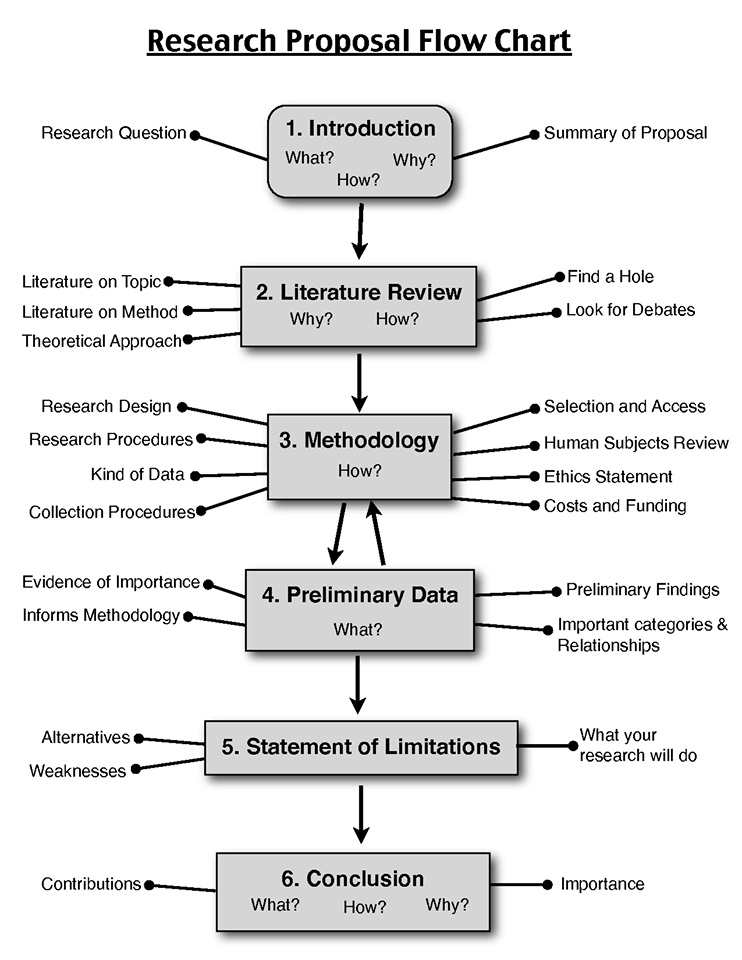
\includegraphics[width=15cm]{Writing research research proposal.png}
	\caption[Research Proposal Flow Chart]
	{The image is a flow chart titled "Research Proposal Flow Chart," designed to guide the development of a research proposal through six key stages: Introduction, Literature Review, Methodology, Preliminary Data, Statement of Limitations, and Conclusion. Each stage addresses specific questions like "What?", "Why?", and "How?", ensuring a comprehensive and structured approach. The chart outlines the progression from defining the research question and reviewing relevant literature, to detailing the methodology, presenting preliminary data, discussing limitations, and concluding with the significance of the research. This visual tool is essential for researchers in planning and articulating their study in a coherent and logical manner.. Figure adapted from \cite{Dorsett2010}.}
	\label{fig:ExxonSpreading}
\end{figure}
%


\subsection{Concept and Terminology Explanation}

In this subsection, you should broadly explain the key concepts and terminology that are central to your research. This will help ensure that readers who are not familiar with the topic can follow along.




\section{ Importance and Relevance} 
\label{SplitScheduleExplain}

In this subsection, explain why the topic is important and relevant. Include statistics, the impact of the topic on society, and any related government policies or initiatives. This helps to justify why your research is necessary and valuable.




\section{Motivation}

The motivation section of a thesis is crucial as it articulates the rationale behind the research, highlighting its importance and relevance. This section will help connects the background information with the research objectives by explaining why the study is necessary and what gaps it aims to fill. 

This section (and its subsection) builds a compelling case for the research by discussing the potential benefits and impact of the findings, thereby justifying the effort and resources invested in the study. The motivation section ensures that the reader understands the significance of the problem being addressed and the value that the proposed solutions can bring to the field.

You can give a brief overview or compact explaination from the literature review, what is there, but what is still missing. or the justification of why you insist of using some technique


\subsection{Some subsection to decompose your explaination}




\section{Problem Formulation}


\subsection{Research Gap}

The identified gap based on your literature review


\subsection{Problem Statement}

Based on the research gap, the following problems have been identified:

\begin{enumerate}
    \item \textbf{Definition of the Problem:} The problem statement clearly defines the issue that the research aims to address. It should describe the gap in knowledge, real-world challenges, or theoretical inconsistencies that necessitate investigation.

    \item \textbf{Relation to Hypotheses:} The problem statement serves as the foundation for formulating hypotheses. It outlines the research issue, while the hypotheses provide testable predictions based on this problem.

    \item \textbf{Best Practices for Writing a Problem Statement:}
    \begin{itemize}
        \item \textbf{Be clear and concise:} The problem statement should be straightforward, avoiding unnecessary jargon while effectively communicating the research issue.
        \item \textbf{Explain the research gap:} Clearly identify what is missing in existing research and why addressing this gap is important.
        \item \textbf{Define the scope:} Specify the boundaries of the problem, ensuring that it is neither too broad nor too narrow.
        \item \textbf{Highlight significance:} Explain why solving this problem is important, including its potential impact on the field, industry, or society.
        \item \textbf{Use evidence to support the problem:} Reference previous studies, statistics, or real-world examples to justify why the problem exists and why it requires investigation.
        \item \textbf{Ensure alignment with research objectives:} The problem statement should align with the study’s aims, ensuring consistency throughout the research process.
    \end{itemize}
\end{enumerate}


\section{Hypotheses of Study}
Based on the depicted problem statement, the following have been hypothesised:

\begin{enumerate}
    \item \textbf{Hypotheses:} A hypothesis is a testable statement or assumption that predicts the relationship between variables in a study. It serves as the foundation for research by providing a direction for investigation.

    \item \textbf{Relation to Problem Statement:} The problem statement defines the research issue and its significance, while hypotheses emerge from it as specific, testable propositions. The hypotheses offer potential explanations or solutions to the problem and guide data collection and analysis.

    \item \textbf{Best Practices for Writing Hypotheses:}
    \begin{itemize}
        \item \textbf{Be clear and specific:} A hypothesis should be precise and unambiguous, defining the variables and their expected relationship.
        \item \textbf{Ensure testability:} A good hypothesis should be measurable and testable using empirical methods.
        \item \textbf{Base it on existing knowledge:} Formulate hypotheses based on prior research, theories, or observations.
        \item \textbf{Use an "If-Then" structure (if applicable):} For causal relationships, use an "If X, then Y" format to establish a clear cause-and-effect relationship.
        \item \textbf{Make it falsifiable:} A hypothesis should be structured in a way that allows it to be proven false if the evidence contradicts it.
        \item \textbf{Keep it simple and focused:} Avoid overly complex hypotheses by keeping them concise and to the point.
    \end{itemize}
\end{enumerate}



\section{Research Question}

\begin{description}
    \item[RQ3] - Is there any significant correlation between social presence and course satisfaction among third-year Malaysian undergraduates undertaking a BL course in UMS?
    \item[RQ4] Is there any significant correlation between cognitive presence and course satisfaction among third-year Malaysian undergraduates undertaking a BL course in UMS?
    \item[RQ5] Which factor of teaching, social, and cognitive presence is dominant in determining course satisfaction among third-year Malaysian undergraduates undertaking a BL course in UMS?
\end{description}

\section{Study Objectives}



Based on the hypotheses, the following research objectives have been formulated:

\begin{enumerate}    
    \item  You may refer to online sources about SMART objectives, which define a goal that is specific, measurable, achievable, relevant, and time-bound.


       


    
\end{enumerate}



\section{Scope Of Work}

The scope of work for this thesis are:

\begin{enumerate}    


	
\end{enumerate}

\section{Organisation Of Thesis}
\label{ThesisOrganisation}


\noindent The organisation of this thesis is elaborated in the following:

Chapter 1 serves as an introduction, providing an overview of the study and emphasizing the importance of ... . You may eloborate more

Chapter 2 discusses relevant background information on.. . You may eloborate more

Chapter 3 details the development of the proposed method. You may eloborate more

Chapter 4 presents the experimental analysis and validation of the proposed . You may eloborate more

Chapter 5 summarizes key findings from each chapter, highlights the research contributions of this thesis in advancing.. You may eloborate more


The Chapter Appendix includes detailed explanations of the s.